%% This Beamer template is based on the one found here: https://github.com/sanhacheong/stanford-beamer-presentation, and edited to be used for Stanford ARM Lab

\documentclass[10pt]{beamer}
%\mode<presentation>{}

\usepackage{media9}
\usepackage{amssymb,amsmath,amsthm,enumerate}
\usepackage[utf8]{inputenc}
\usepackage{array}
\usepackage[parfill]{parskip}
\usepackage{graphicx}
\usepackage{caption}
\usepackage{subcaption}
\usepackage{bm}
\usepackage{amsfonts,amscd}
\usepackage[]{units}
\usepackage{listings}
\usepackage{multicol}
\usepackage{multirow}
\usepackage{tcolorbox}
\usepackage{physics}
%encoding
%--------------------------------------
\usepackage[T1]{fontenc}
\usepackage[utf8]{inputenc}
%--------------------------------------

%Portuguese-specific commands
%--------------------------------------
\usepackage[portuguese]{babel}
%--------------------------------------

%Hyphenation rules
%--------------------------------------
\usepackage{hyphenat}
\hyphenation{mate-mática recu-perar}
%--------------------------------------

% Enable colored hyperlinks
\hypersetup{colorlinks=true}

% The following three lines are for crossmarks & checkmarks
\usepackage{pifont}% http://ctan.org/pkg/pifont
\newcommand{\cmark}{\ding{51}}%
\newcommand{\xmark}{\ding{55}}%

% Numbered captions of tables, pictures, etc.
\setbeamertemplate{caption}[numbered]

%\usepackage[superscript,biblabel]{cite}
\usepackage{algorithm2e}
\renewcommand{\thealgocf}{}

% Bibliography settings
\usepackage[style=ieee]{biblatex}
\setbeamertemplate{bibliography item}{\insertbiblabel}
\addbibresource{references.bib}

% Glossary entries
\usepackage[acronym]{glossaries}
\newacronym{ML}{ML}{machine learning}
\newacronym{HRI}{HRI}{human-robot interactions}
\newacronym{RNN}{RNN}{Recurrent Neural Network}
\newacronym{LSTM}{LSTM}{Long Short-Term Memory}


\theoremstyle{remark}
\newtheorem*{remark}{Remark}
\theoremstyle{definition}

\newcommand{\empy}[1]{{\color{darkorange}\emph{#1}}}
\newcommand{\empr}[1]{{\color{cardinalred}\emph{#1}}}
\newcommand{\examplebox}[2]{
\begin{tcolorbox}[colframe=darkcardinal,colback=boxgray,title=#1]
#2
\end{tcolorbox}}

\usetheme{Stanford} 
\def \i  {\item}
\def \ai {\item[] \quad \arrowbullet}
\newcommand \si[1]{\item[] \quad \bulletcolor{#1}}
\def \wi {\item[] \quad $\ \phantom{\Rightarrow}\ $}
\def \bi {\begin{itemize}\item}
\def \ei {\end{itemize}}
\def \be {\begin{equation*}}
\def \ee {\end{equation*}}
\def \bie {$\displaystyle{}
\def \eie {{\ }$}}
\def \bsie {\small$\displaystyle{}
\def \esie {{\ }$}\normalsize\selectfont}
\def \bse {\small\begin{equation*}}
\def \ese {\end{equation*}\normalsize}
\def \bfe {\footnotesize\begin{equation*}}
\def \efe {\end{equation*}\normalsize}
\renewcommand \le[1] {\\ \medskip \lefteqn{\hspace{1cm}#1} \medskip}
\def \bex {\begin{example}}
\def \eex {\end{example}}
\def \bfig {\begin{figure}}
\def \efig {\end{figure}}
\def \btheo {\begin{theorem}}
\def \etheo {\end{theorem}}
\def \bc {\begin{columns}}
\def \ec {\end{columns}}
\def \btab {\begin{tabbing}}
\def \etab {\end{tabbing}\svneg\svneg}
\newcommand \col[1]{\column{#1\linewidth}}
\def\vneg  {\vspace{-5mm}}
\def\lvneg {\vspace{-10mm}}
\def\svneg {\vspace{-2mm}}
\def\tvneg {\vspace{-1mm}}
\def\vpos  {\vspace{5mm}}
\def\lvpos {\vspace{10mm}}
\def\svpos {\vspace{2mm}}
\def\tvpos {\vspace{1mm}}
\def\hneg  {\hspace{-5mm}}
\def\lhneg {\hspace{-10mm}}
\def\shneg {\hspace{-2mm}}
\def\thneg {\hspace{-1mm}}
\def\hpos  {\hspace{5mm}}
\def\lhpos {\hspace{10mm}}
\def\shpos {\hspace{2mm}}

\logo{
\includegraphics[height=0.4in]{./images/logoufjf10.png}}

% commands to relax beamer and subfig conflicts
% see here: https://tex.stackexchange.com/questions/426088/texlive-pretest-2018-beamer-and-subfig-collide
\makeatletter
\let\@@magyar@captionfix\relax
\makeatother

\newcommand{\code}[1]{\textcolor{red} {\textit{#1}}} %comentarios

\title[Reunião de Orientação 03]{Reunião de Orientação 03}
%\subtitle{Subtitle Of Presentation}

%\beamertemplatenavigationsymbolsempty

\begin{document}

\author[Modelagem Computacional]{
	\begin{tabular}{c} 
	\Large
	Igor Pires dos Santos\\
    \footnotesize \href{mailto:igor.pires@ice.ufjf.br}{igor.pires@ice.ufjf.br}\\
    \textbf{Orientador:} Rafael Bonfim
\end{tabular}
\vspace{-4ex}}

\institute{
	\vskip 5pt
	\begin{figure}
		\centering
		\begin{subfigure}[t]{0.5\textwidth}
			\centering
			
\includegraphics[height=0.33in]{images/logoufjf1}
		\end{subfigure}%
		~ 
		\begin{subfigure}[t]{0.5\textwidth}
			\centering
			
\includegraphics[height=0.33in]{./images/PGMC.png}
		\end{subfigure}
	\end{figure}
	\vskip 5pt
	Programa de Pós-Graduação em Modelagem Computacional\\
	Universidade Federal de Juiz de Fora\\
	\vskip 3pt
}

% \date{June 15, 2020}
\date{\today}

\begin{noheadline}
\begin{frame}\maketitle\end{frame}
\end{noheadline}

\setbeamertemplate{itemize items}[default]
\setbeamertemplate{itemize subitem}[circle]

\begin{frame}
	\frametitle{Sumário} % Table of contents slide, comment this block out to remove it
	\tableofcontents % Throughout your presentation, if you choose to use \section{} and \subsection{} commands, these will automatically be printed on this slide as an overview of your presentation
\end{frame}

\section{Introdução}
\begin{frame}[allowframebreaks]
\frametitle{Avanços}

	\begin{itemize}
		\item \textbf{Matérias do Mestrado: } Como combinado nesse período eu foquei nas matérias restantes do mestrado, Eng. de Software e Plataformas Computacionais. Estas matérias estão acabando hoje também no dia 02/10.
		
		\item \textbf{Engenharia de Software: }Como também mencionado eu foquei no ambiente do Docker que seria utilizado para compilar o IGU em um ambiente multiplataforma.
		
		\item \textbf{Plataformas Computacionais: }Esta matéria foi feita em cima da plataforma \textit{Abaqus CAE} que é uma ferramenta complexa utilizada na simulação de problemas mecânicos.
	\end{itemize}
	
	\framebreak
	
	\begin{center}
		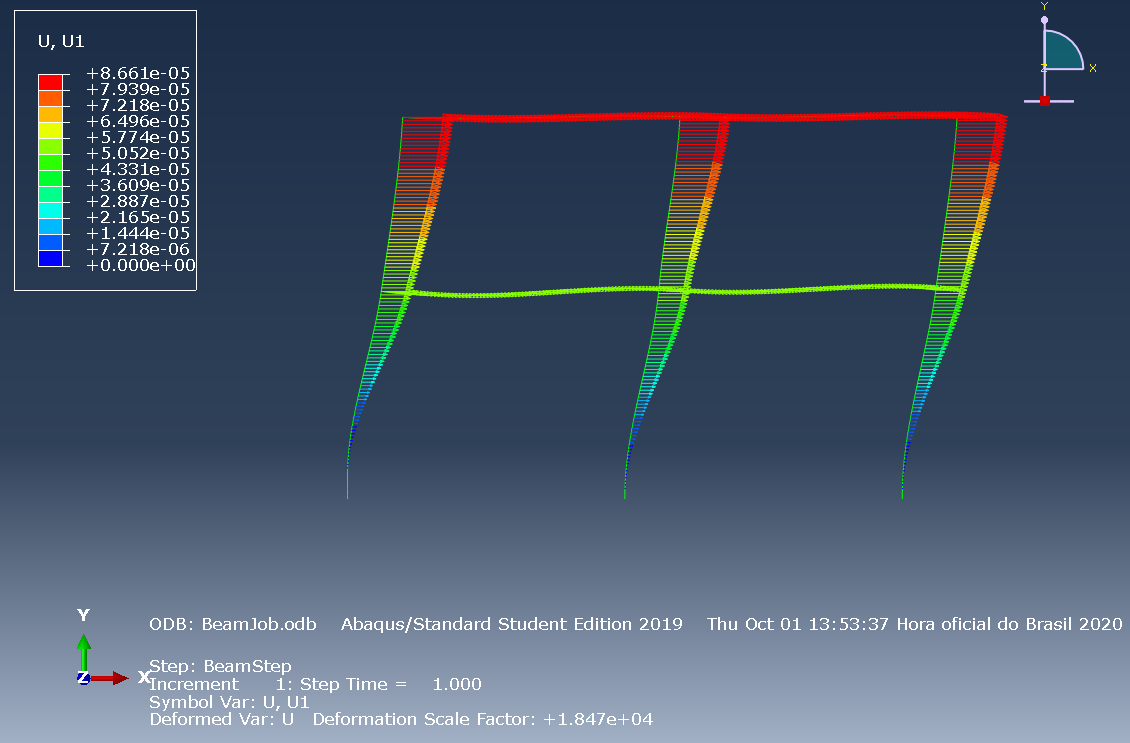
\includegraphics[width=0.7\textwidth]{images/004.png}
	\end{center}
	
	\framebreak
	
	\begin{center}
		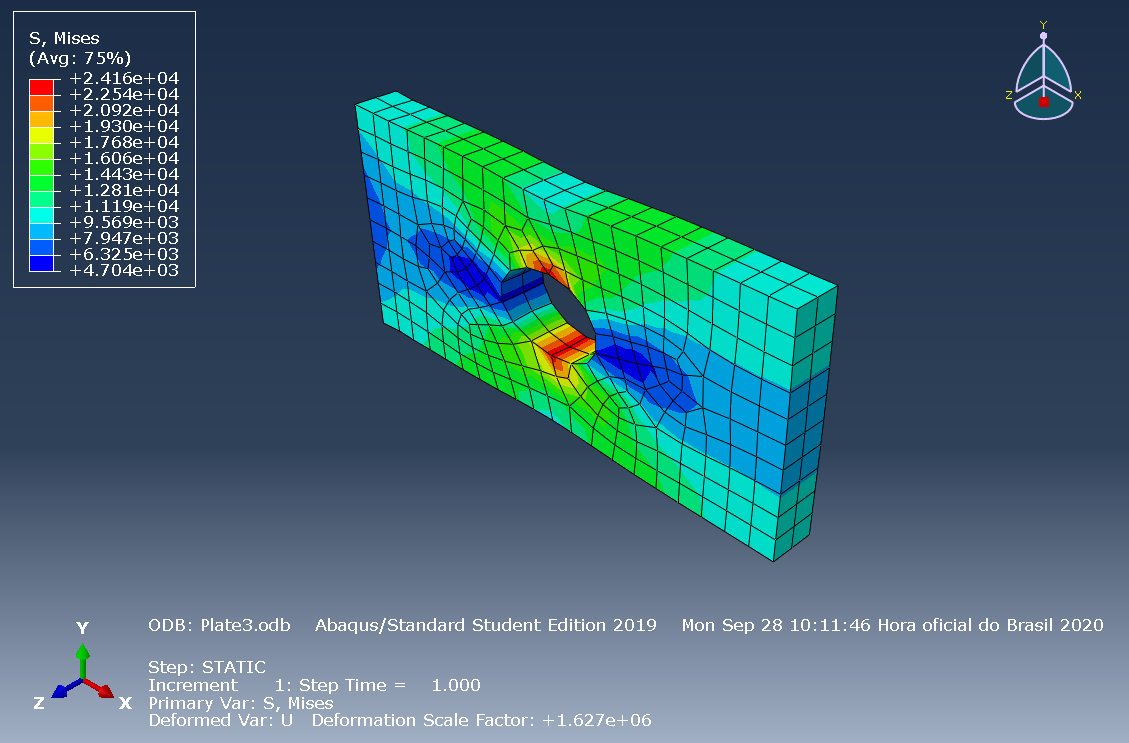
\includegraphics[width=0.7\textwidth]{images/007.png}
	\end{center}
	
	\framebreak
	
	\begin{itemize}

		\item \textbf{Engenharia de Software}
		
		\item Essa matéria foi lecionada no modelo ERE do PGMC que apresentou alguns novos desafios, por isso a matéria teve uma profundidade menor, mas o que não impediu que eu pesquisasse mais sobre o Docker.
		
		\item Como mencionado anteriormente, o Docker é uma ferramenta que se baseia em imagens, imagens estas que possuem todos os arquivos e configurações de ambiente similar à uma máquina virtual. Entretanto o Docker é muito mais poderoso pois faz isso sem o processo de virtualização, sendo muito mais rápido.
		
		\item O docker é algo que venho pesquisando desde o final do ano passado e agora finalizei um curso sobre o uso dele em conjunto com a ferramenta de CI/CD Jenkins e Atlassian Bamboo.
		
	\end{itemize}
	
	\framebreak
	
	\begin{center}
		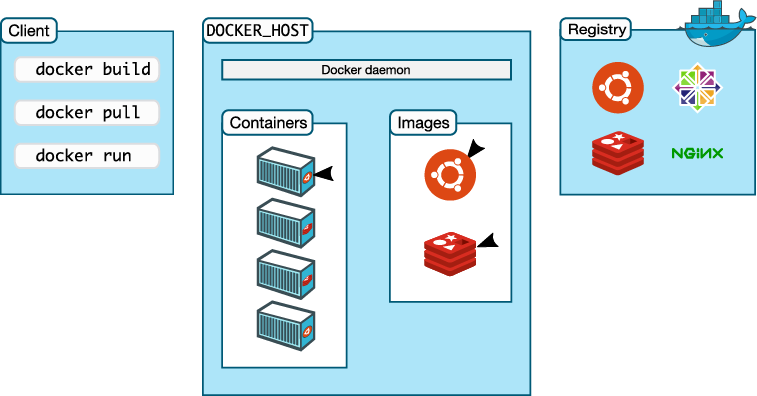
\includegraphics[width=0.7\textwidth]{images/01.png}
	\end{center}
	
	
	\framebreak
	
	\begin{itemize}
		\item Utilizando o ambiente do Docker é possível contruir essas imagens personalizadas, portanto eu construí um repositório da imagem do Ubuntu com a biblioteca Qt e as bibliotecas adicionais do OpenGL entitulado mrblackpower/ubuntuqt
		
		\item \href{https://hub.docker.com/repository/docker/mrblackpower/ubuntuqt}{https://hub.docker.com/repository/docker/mrblackpower/ubuntuqt}
		
		\item Equivalente ao repositório Bitbucket:
		
		\item \href{https://bitbucket.org/MrBlackPower/ubuntuqt/src/main/}{https://bitbucket.org/MrBlackPower/ubuntuqt/src/main/}
	\end{itemize}
	
	\framebreak
	
	\begin{itemize}
		\item \textbf{O ciclo de vida de um software}
		
	\end{itemize}
	
	\begin{center}
		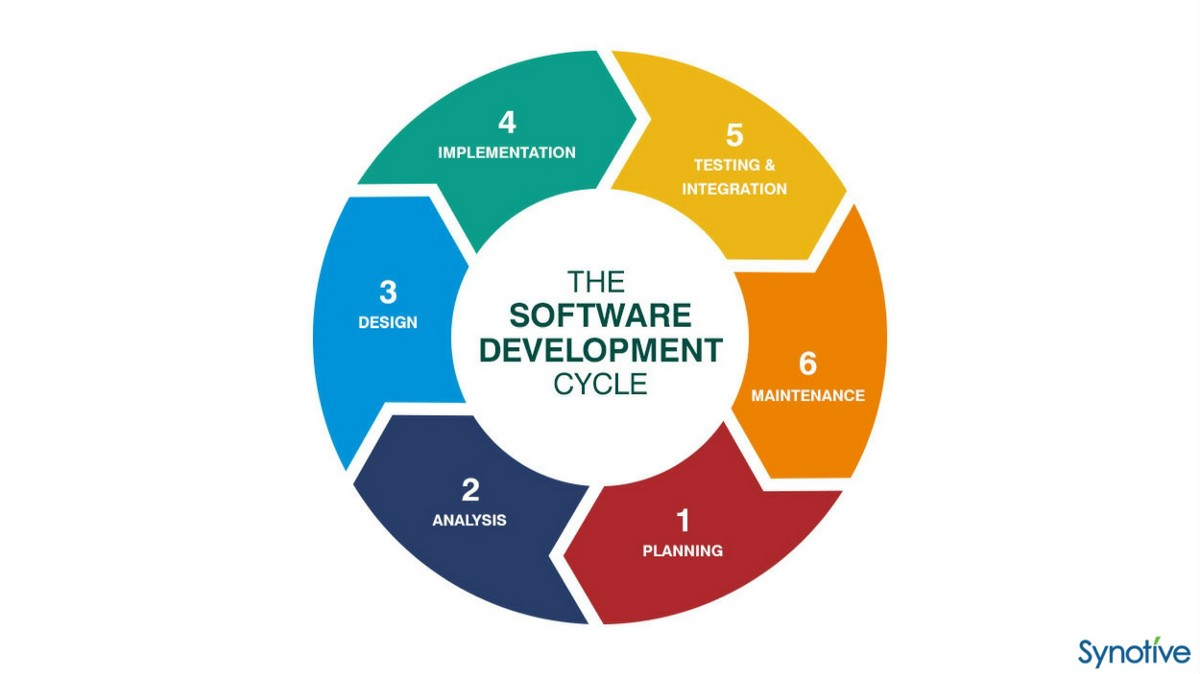
\includegraphics[width=0.7\textwidth]{images/05.jpg}
	\end{center}
	
	\framebreak
	
	\begin{itemize}
		\item \textbf{Continuous Integration}
		
		\item O processo de CI (Continuour Integration) consiste na integração de funcionalidades "recém-criadas" continuamente.
		
		\item Por exemplo, foi desenvolvida uma ferramenta que resolve o fluxo pulsátil utilizando diferentes resolvedores e compara os resultados. Um destes resolvedores ainda está em "desenvolvimento" e se deseja que esta funcionalidade seja integrada contínuamente ao sistema para evitar problemas de integração.
		
	\end{itemize}
	
	\framebreak
	
	\begin{itemize}
		\item \textbf{O que é Integrar?}
		
		\item A definição exata do processo de integração varia de software para software, mas em geral é o processo de compilação. Em um projeto C++ comum, integrar contínuamente seria executar os testes unitários e compilar o código, caso o processo falhe é gerado um alerta.
		
	\end{itemize}
	
	\framebreak
	
	\begin{itemize}
		\item \textbf{Continuous Delivary}
		
		\item O processo de CD (Continuour Delivery) consiste na entrega de funcionalidades "recém-criadas" continuamente.
		
		\item Por exemplo, a mesma ferramenta que resolvedora utilizando diferentes resolvedores. O resolvedor é integrado contínuamente e se deseja que esta funcionalidade seja entregue contínuamente ao cliente.
		
	\end{itemize}
	
	\framebreak
	
	\begin{itemize}
		\item \textbf{O que é Entregar?}
		
		\item A definição exata do processo de entrega varia de software para software, mas em geral é o processo de instalar o software na máquina. Em um projeto C++ comum, a entrega contínua seria a geração do artefato (ou executável), caso o processo falhe na criação ou inicialização é gerado um alerta.
		
	\end{itemize}
\end{frame}

\section{Primeiro Problema}
\begin{frame}[allowframebreaks]
\frametitle{Primeiro Problema}
	\begin{itemize}
	
		\item \textbf{O Problema}: Apesar de utilziar o mesmo SO, o mesmo compilador e as mesmas bibliotecas as versões diferiam, com isso algumas funções deixavam de ser suportadas e outras surgiam. Portanto, diversas vezes as mudanças eram criadas no programa e não era possível "integrá-las" ao ambiente externo. 
		
		\item \textbf{A Solução}: Utilizar um contêiner como ambiente padrão de desenvolvimento \textbf{OU} utilizar mais de um contêiner com as versões aceitas definidas.

		\item \textbf{Antes}: Compilava no sistema local, rezava antes de compilar em outro lugar.
		
	\end{itemize}
\end{frame}
	

\section{Docker}
\begin{frame}[allowframebreaks]
\frametitle{Docker}
	
	\begin{itemize}
		\item \textbf{Papel do Docker}
		
		\item Conforme mencionado anteriormente o Docker é um repositório de imagens que são executadas em contêineres. Contêineres estes que podem ser executados nos mais diversos ambientes e que possuem definições próprias do seu ambiente interno. Portanto, através do Docker é possível se padronizar o ambiente em que esta integração e entega ocorrerão.
	\end{itemize}
	
	\framebreak
	
	\begin{itemize}
		\item O mais interessante do Docker é que ele funciona em conjunto com as tecnologias já existentes para CI/CD, podendo ser utilizado em partes ou em todo o processo.
		\item Com ferramentas automatizadoras como o Jenkins e o Atlassian Bamboo é possível utilizar contêineres internas à estas ferramentas que executarão os testes, compilarão o código, armazerarão os artefatos e entregarão estes artefatos.		
		
	\end{itemize}
	
	\framebreak
	
	\begin{center}
		
\includegraphics[width=0.7\textwidth]{images/38.png}
	\end{center}
	
	\begin{center}
		
\includegraphics[width=0.7\textwidth]{images/39.png}
	\end{center}
	
	\framebreak
	
	\begin{itemize}

		\item Aplicar o conceito de CI \& CD efetivamente é realizar todos os passos que você (o programador, o analista de sistema ou devOps) executa após terminar a edição do código de forma automática e/ou periódica.
		
		\item Assim como o git, o Bamboo e o Jenkins são servidores que rodam contínuamente. Estes automatizadores recebem sinais de "gatilhos" (\textit{hooks}) ou realizam chamadas periodicamente. Estes servidores são capazes de utilizar as tecnologias de repositório do git e a contêinerização do docker.
		
		\item Isto é, ao enviar o código para o repositório um gatilho é ativo e recebido pelo automatizador, que por sua vez envia o código fonte aos contêineres e realiza as ações através de comandos CLI ou Powershell. É possível ainda utilizar protocolos adjacentes como SSH e o SCP que permitem a utilização de recursos na mesmarede.
		
	\end{itemize}
	
	\framebreak
	
	\begin{itemize}
	
		\item Ambas a ferramentas de CI/CD aqui citadas foram desenvolvidas em Java utilizando Apache Tomcat e JDK, sendo o Jenkins Open Source. Logo, ambas as soluções podem ser utilizadas sem o Docker.
		
		\item Entretanto, é extremamente fácil utilizar estas ferramentas em união com o Docker. Ambas a ferramentas possuem imagens no repositório com os servidores e podem ser iniciadas com:
		
		\item \code{docker container run atlassian/bamboo-server}
		
		\item \code{docker container run jenkins/jenkins}
		
	\end{itemize}
	
	\framebreak
	
	\begin{itemize}
	
		\item Com estes comandos os servidores são criados, entretanto é necessária a configuração dos \textit{volumes} para que os dados configurados sejam persistidos em disco corretamente.
		
	\end{itemize}
	
	\begin{center}
		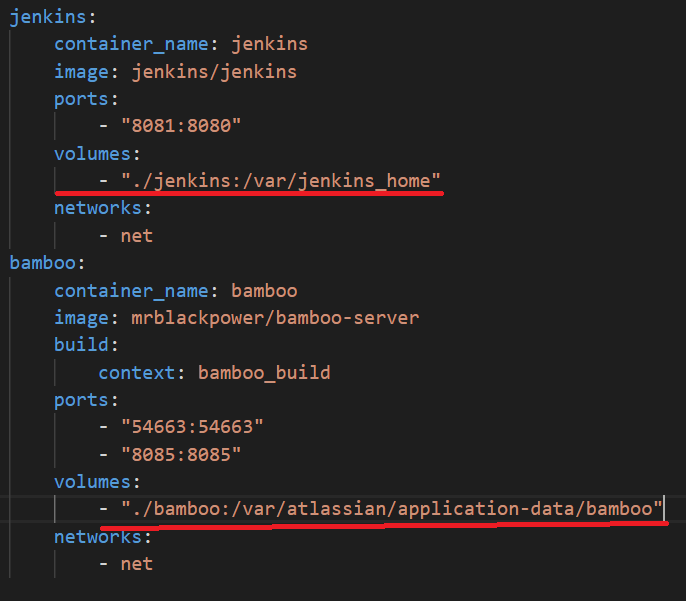
\includegraphics[width=0.7\textwidth]{images/41.png}
	\end{center}
	
	\framebreak
	
	\begin{center}
		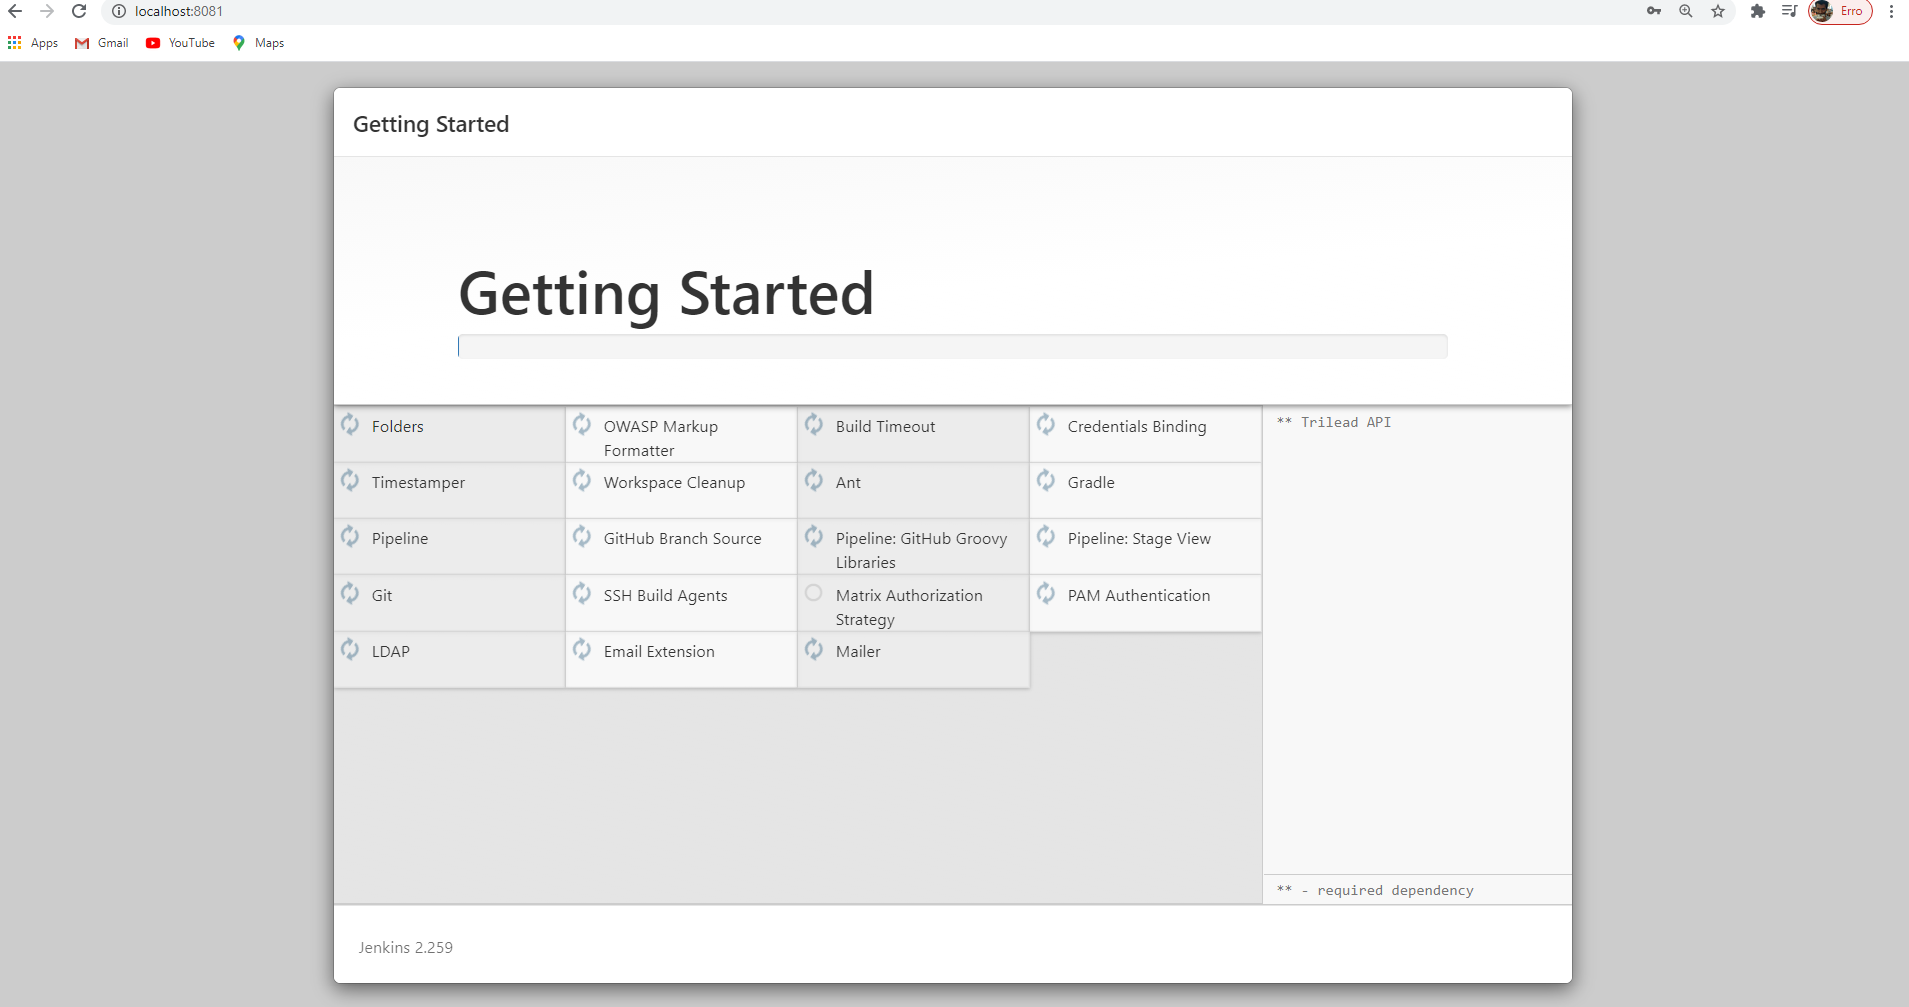
\includegraphics[width=0.7\textwidth]{images/42.png}
	\end{center}
	
	\framebreak
	
	\begin{itemize}
	
		\item Com isto os servidores rodam e têm suas portas expostas. Assim como um servidor git os srvidores de CI/CD possuem projetos e contas de usuários. Estas contas são utilizadas pelos servidores para gerenciar qual usuário tem acesso à qual projeto e quais permissões sobre o projeto.
		
		\item Isto é extremamente útil para empresas e softwares maiores, pois um processo de deployment significaria uma mudança em servidor que não poderia e nem deveria ser feita por um grande número de pessoas.
		
	\end{itemize}
	
\end{frame}

\section{Segundo Problema}
\begin{frame}[allowframebreaks]
\frametitle{Segundo Problema}
	\begin{itemize}
	
		\item \textbf{O Problema}: Após o processo de compilação gostaria de se entregar efetivamente o executável gerado. 
		
		\item \textbf{A Solução}: Compilar o código-fonte dentro do contêiner e enviar artefato à nuvem \textbf{OU} envia artefatos para outro lugar.
		
		\item \textbf{Antes}: Mesmo processo, entretanto manualmente.
		
	\end{itemize}
\end{frame}

\section{Docker Cloud Services}
\begin{frame}[allowframebreaks]
\frametitle{Docker Cloud Services}
	\begin{itemize}
	
		\item Utilizando imagens Unix é possível instalar os serviços AWS (\textit{Amazon Web Services} e GCP (\textit{Google Cloud Platform}) que possibilitam o envio destes artefatos à nuvem instantâneamente.
		
		\item A grande vantagem de utilizar estes serviçoes da nuvem é que eles podem ser consumidos de qualquer lugar com acesso à internet.
		
	\end{itemize}
\end{frame}

\section{Terceiro Problema}
\begin{frame}[allowframebreaks]
\frametitle{Terceiro Problema}
	\begin{itemize}
	
		\item \textbf{O Problema}: Tá, fiz isso tudo, mas agora quero fazer multiplataforma (Linux + Window). 
		
		\item \textbf{A Solução}: Utilizar Docker in Docker \textbf{OU} Docker beside Docker com as imagens de SO desejadas.
		
		\item \textbf{Antes}: Se você compilar roda...
		
	\end{itemize}
\end{frame}

\section{Docker Mutilayer}
\begin{frame}[allowframebreaks]
\frametitle{Docker Mutilayer}
	
	\begin{center}
		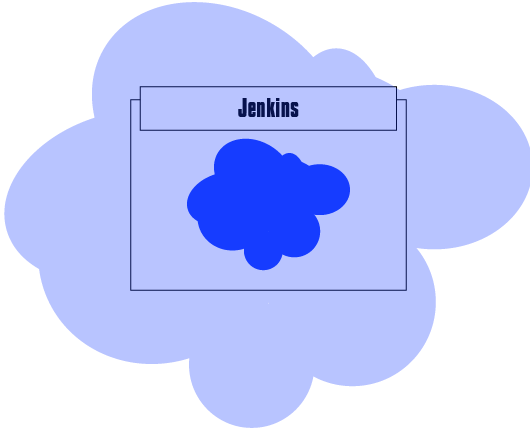
\includegraphics[width=0.7\textwidth]{images/40.png}
	\end{center}
	
	\framebreak
	
	\begin{itemize}
	
		\item Docker beside Docker consistem em utilizar contêineres docker ao lado do contêiner que contém o servidor de CI/CD. Desta forma os comandos são executados internamente dos contêineres adjacentes através da rede definida entre eles utilizando os protocolos já conhecidos, como SSH e SCP.
		
		\item É possível utilizar esta tecnologia também sem utilizar o servidor CI/CD dentro de um contêiner mas localmente. Basta abrir as portar locais corretamente e configurar o servidor CI/CD com o endereço local ao invés do endereço do contêiner.
		
	\end{itemize}
	
	\framebreak
	
	\begin{center}
		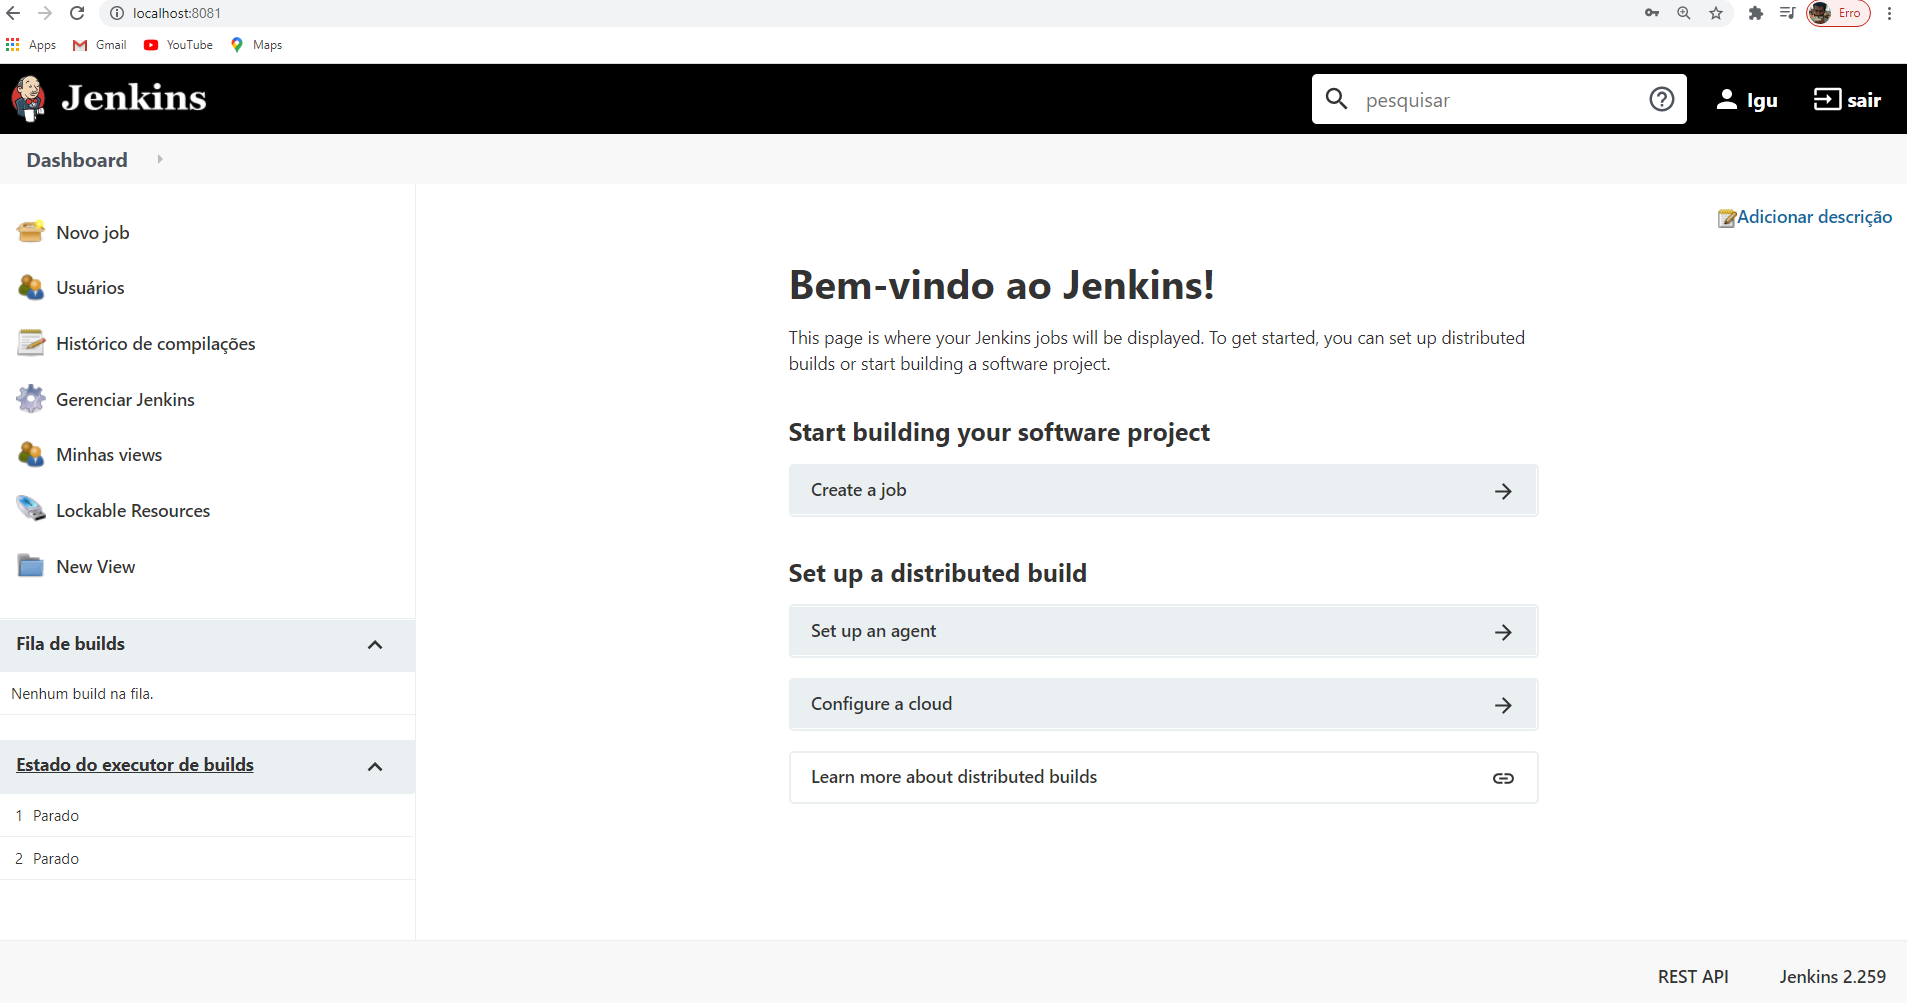
\includegraphics[width=0.7\textwidth]{images/43.png}
	\end{center}
	
	\framebreak
	
	\begin{itemize}
		\item 	Plugins
	\end{itemize}
	
	\begin{center}
		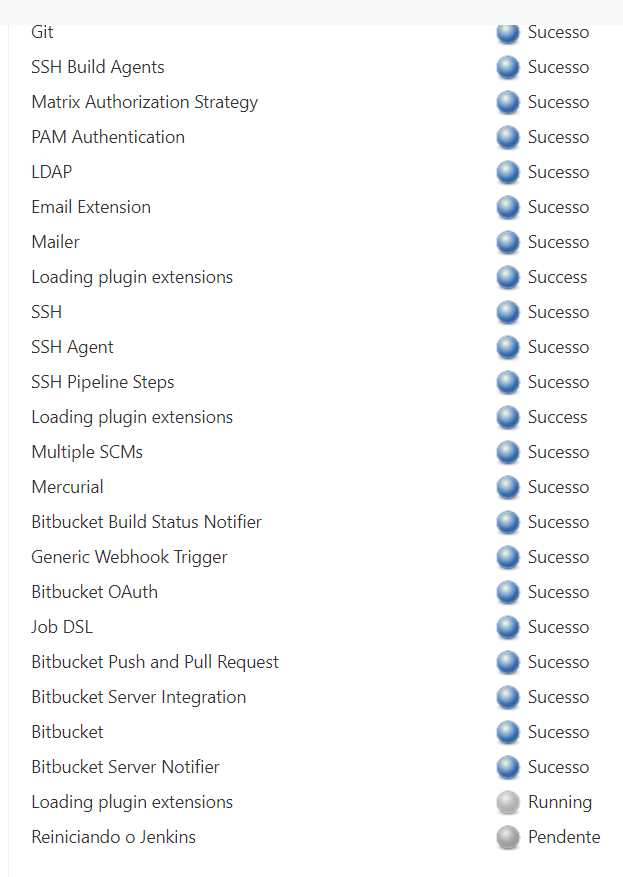
\includegraphics[width=0.3\textwidth]{images/44.png}
	\end{center}
	
	\framebreak
	
	\begin{center}
		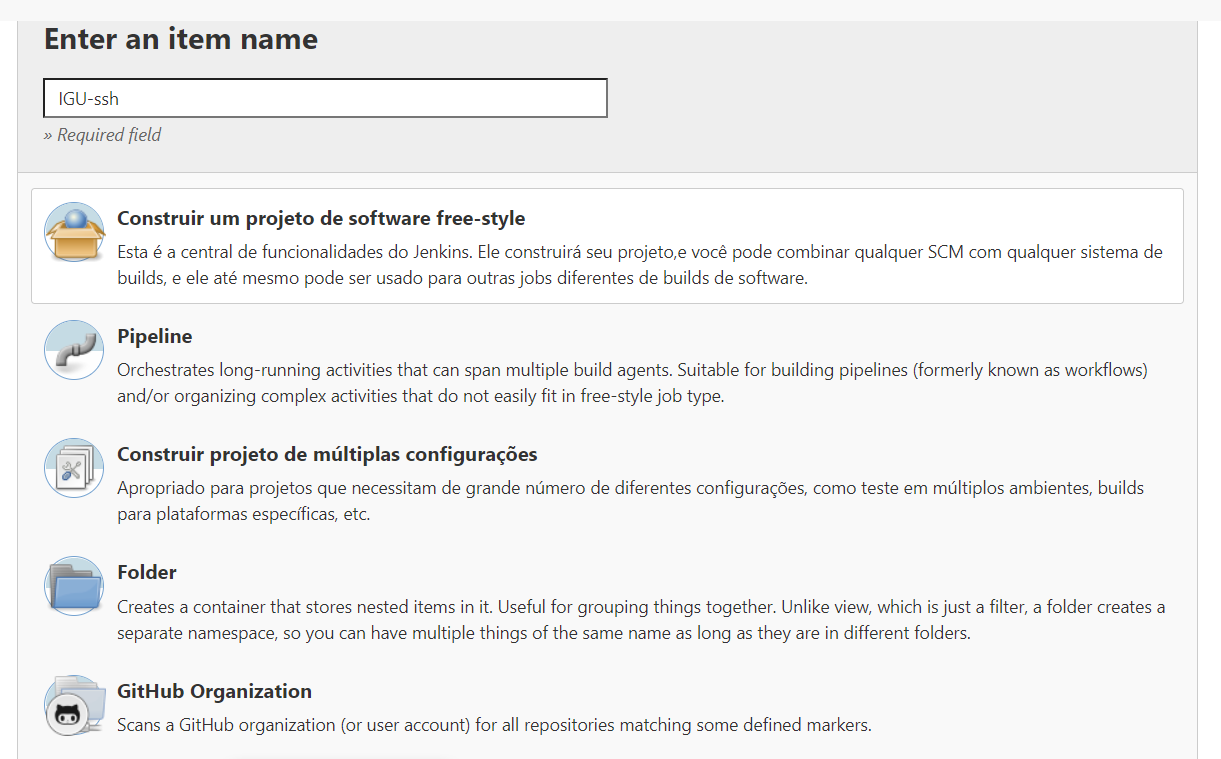
\includegraphics[width=0.7\textwidth]{images/45.png}
	\end{center}
	
	\framebreak
	
	\begin{center}
		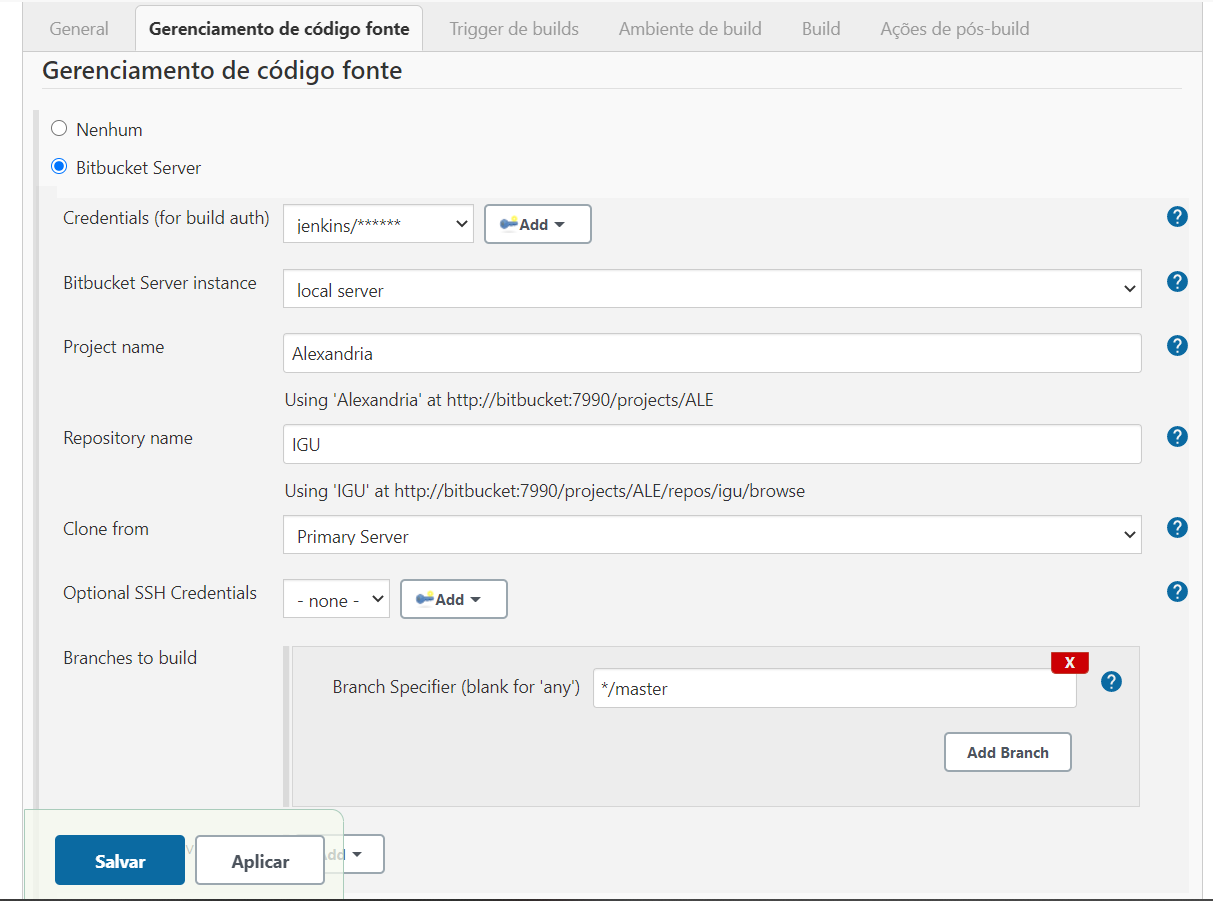
\includegraphics[width=0.7\textwidth]{images/46.png}
	\end{center}
	
	\framebreak
	
	\begin{center}
		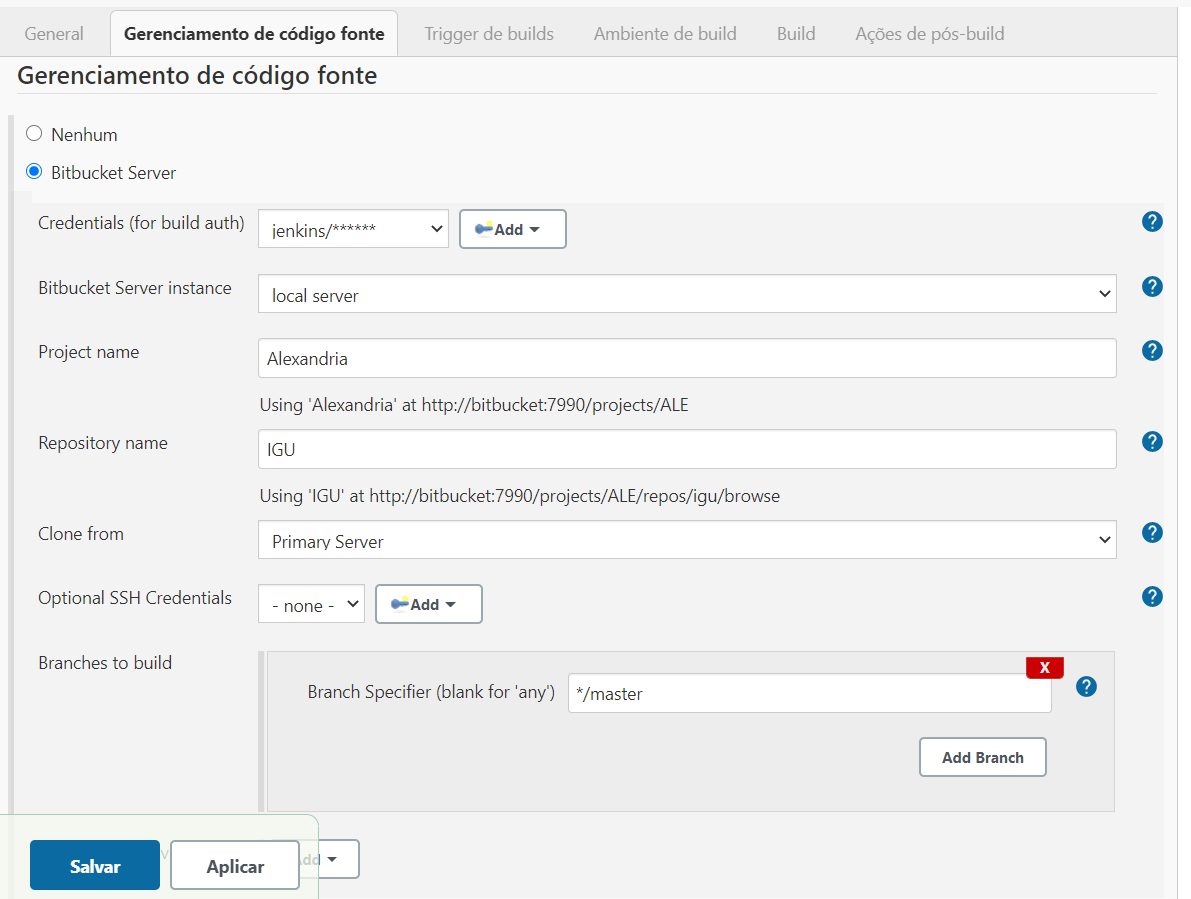
\includegraphics[width=0.7\textwidth]{images/47.png}
	\end{center}
	
	\framebreak
	
	\begin{itemize}
	
		\item Além de toda essa configuração é necessário também configurar o servidor SSH rodando no contêiner de destino, tal configuração é feita na construção do contêiner.
	
		\item O problema com Docker beside Docker é que contêineres Windows não rodam com o mesmo suporte que contêineres Unix, isto é, é possível rodar contêineres Unix ou contêineres Windows, mas não ambos ao mesmo tempo.
		
	\end{itemize}
	
	\framebreak
	
	\begin{itemize}
	
		\item Docker in Docker consistem em utilizar contêineres docker dentro do contêiner que contém o servidor de CI/CD. Desta forma os comandos são executados internamente dos contêineres.
		
		\item É possível utilizar esta tecnologia também sem utilizar o servidor CI/CD dentro de um contêiner mas localmente. Basta ter o Docker e o servidor de CI/CD instalado no mesmo ambiente.
		
	\end{itemize}
	
	\framebreak
	
	\begin{itemize}
	
		\item (mostrar ambiente com Jenkins e Bamboo)
		
		\item Novos paradigmas, novos problemas!
		
	\end{itemize}
	
	\framebreak
	
	\begin{itemize}
		\item \textbf{Problemas: } 

		\item Compilar em um mesmo computador contêineres Windows e Unix está se provando cada vez mais difícil, entretanto descobri que não é necessariamente preciso, porque do linux tem como compilar para o Windows, mas é igualmente complicado (AppImages).
		
		\item Mas é possível disponibilizar uma imagem com o IGU instalado e sendo utilizado através da linha de comando.
	\end{itemize}
	
	
	\framebreak
	
	\begin{itemize}
		\item \textbf{Proposta Anterior} 
		\item Utilizar o IGU "1.0" para realizar os estudos de caso
		\item Criar as ferramentas do IGU "2.0" (as mesmas presentes no IGU "1.0" adicionadas ao paradigma Paralelismo, Interface Atualizada, Linha de Comando, Programa Distribuído).
		
		
	\end{itemize}
	
	
	\framebreak
	
	\begin{itemize}
		\item \textbf{Proposta Atual}
		\item Outubro: Realização do Toefl iBT, Adicionar possibilidade de se executar o IGU 1.0 via linha de comando, Finalizar Repositório de imagem com o IGU 1.0 Instalado, Definir os experimentos relevantes com CCO (Ye, Pressão e Fluxo?)(Quais parâmetros ?), Definir se um sistema de CI/CD será aplicado e QUAL e COMO.
		
		\item Novembro: Finalização da Graduação, Rodar os experimentos relevantes com CCO utilizando o IGU 1.0 , escrever (e plotar) estes resultados.
		
		\item Dezembro: Finalizar parte Gráfica IGU 2.0, finalizar sistema de CI/CD, re-analisar funcionalidades do IGU 2.0 à adicionar e começar dissertação.
		
		\item Janeiro: Começar IGU 2.0 e sua parte distribuída e escrever dissertação.
		
		\item Fevereiro: Finalizar IGU 2.0 e sua parte distribuída, extrair resultados e escrever dissertação.
		
		\item Março: Escrever dissertação.
		
		\item Abril: $??$
		
		\item Maio: $??$
		
		\item Junho: $??$
		
	\end{itemize}
	
	
	\framebreak
	
	\begin{itemize}
	\item Dúvidas:
	
	\item Qual a linha de pesquisa eu devo procurar quando estiver procurando instituições da Alemanha de pesquisa$?$
	
	\end{itemize}
	
\end{frame}

\end{document}